%----------------------------------------------------------------------------------------
%	Metropolia Thesis LaTeX Template
%----------------------------------------------------------------------------------------
% License:
% This work is licensed under the Creative Commons Attribution 4.0 International License. To view a copy of this license, visit http://creativecommons.org/licenses/by/4.0/.
%
% Authors:
% Panu Leppäniemi, Patrik Luoto and Patrick Ausderau
%
% Credits:
% Panu Leppäniemi: abstract, def, cleaning,...
% Patrik Luoto: title page, abstract in Finnish, abbreviation, math,...
% Patrick Ausderau: initial version, style, table of content, bibliography, figure, appendix, table, source code listing...
%
% Please:
% If you find mistakes, improve this template and alike, please contribute by sharing your improvements and/or send us your feedback there: https://github.com/panunu/metropolia-thesis-latex
% And of course, if you improve it, add yourself as an author.
%
% Compiler:
% Use XeLaTeX as a compiler.

%----------------------------------------------------------------------------------------
%    ToDo
%----------------------------------------------------------------------------------------
% % % TÄRKEÄT
% % Translate "listing" in finnish (when inserting source code in the text)
% % Joku ifdef-tyyppinen vipu kieliversiolle (otsikot ja placeholdertekstit)
%    % Vaihtoehtona tietty erilliset filet suomelle ja enkulle, mutta
%    % tämä heikentää päivitettävyyttä (pitää aina muistaa korjata kahteen paikkaan).
%    % PA: I put CAPS comments where to switch depending on the language
% % Lisensointi (otsikkoon tekijä ja avoin lisenssi (esim. CC-BY, pohjan laatija
%   mainittava kommenttirivillä tjsp. [pohja ei ylitä teoskynnystä mutta kiva mainita].
%   PA: done
% % Projektin siirto Githubiin (siinä on issueträkkäys sun muut kivasti kunnossa) Vai?
%   %PA: done
% % Odotetaan 29.11.2013 asti äikänmaikkojen ja viestinnän mahdollisia kommentteja.
%   %done?
% %Reduce the vertical spacing for appendix in table of content
%   %done
%
% % % Vähemmän tärkeät
  % PNG:iden tilalle vektorigraffaa, jos vain löytyy kohtuuvaivalla

 
%----------------------------------------------------------------------------------------
%	THESIS
%----------------------------------------------------------------------------------------

\author{Joonas Paavola}
\title{Loppukäyttäjän antenniratkaisut mobiiliverkon datasovelluksissa}

%IN ENGLISH, you can comment out/remove till line \def\avainsanat
\def\otsikko{Otsikko}
\def\pvm{\ddmmyyyydate\today}
\def\tutkinto{Tutkinto}
\def\kohjelma{Koulutusohjelma}
\def\suuntautumis{Suuntautumisvaihtoehto}
\def\ohjaajat{Ohjaajat}
\def\avainsanat{avainsana}
\date{\today}
\def\metropoliadegree {Bachelor of Engineering}
\def\metropoliadegreeprogramme {Name of your degree programme}
\def\metropoliaspecialisation {Name of your specialisation option}
\def\metropoliainstructors {
First name Last name, Title (for example: Project Manager)\newline
First name Last name, Title (for example: Principal Lecturer)
}
\def\metropoliakeywords {Keywords}

%----------------------------------------------------------------------------------------
%	GLOBAL STYLES
%----------------------------------------------------------------------------------------

\documentclass[11pt,a4paper,oneside,article,finnish]{memoir}
%\usepackage[utf8]{inputenc}
\usepackage[ansinew]{inputenc}
\usepackage[T1]{fontenc}
\usepackage[finnish]{babel} %change this depending on your language
\usepackage{amsmath}
\usepackage{amsfonts}
\usepackage{amssymb}
\usepackage{fontspec}
\usepackage{tocloft}
%\usepackage{lipsum}
\usepackage{titlesec}
\usepackage[hyphens]{url}
\usepackage{mathtools}
\usepackage{wallpaper}
\usepackage{eso-pic}
\usepackage{datetime}
%\usepackage{lastpage} %other trick ;)
\usepackage{url}
\usepackage[amssymb]{SIunits}


\usepackage{float}



\renewcommand{\dateseparator}{.}
%condition for adding or not space in TOC
\usepackage{etoolbox}
%for compact list
\usepackage{enumitem}
%for block comment
\usepackage{verbatim}
%for "easier" references
\usepackage{varioref}
%forcing single line spacing in bibliography
\DisemulatePackage{setspace}
\usepackage{setspace}
%including figure (image)
\usepackage{graphicx}
%change the numbering for figure
\usepackage{chngcntr}
%strike trough
\usepackage{ulem}
%euro symbol
\usepackage{eurosym}
%try to count
\usepackage{totcount}
%insert source code
\usepackage{listings}
\usepackage{caption}
\usepackage{color}
%force the width of a table instead of column
\usepackage{tabularx}

%NORMAL TEXT
%all text, title, etc. in the same font: Arial
\setmainfont{Arial}
%line space
\linespread{1.5}
%\doublespacing
%margin
\usepackage[top=2.5cm, bottom=3cm, left=4cm, right=2cm, nofoot]{geometry}
\setlength{\parindent}{0pt} %first line of paragraph not indented
\setlength{\parskip}{16.5pt} %one empty line to separate paragraph
%list with small line space separation
\tightlists

%IMAGE - FIGURE
%the figures should be placed in the "illustration" folder
\graphicspath{{illustration/}}
%figure number without chapter (1.1, 1.2, 2.1) to (1, 2, 3)
\counterwithout{figure}{chapter}
%border around images
\setlength\fboxsep{0pt}
\setlength\fboxrule{0.5pt}
%caption font size
\captionnamefont{\small}
\captiontitlefont{\small}
%space after figure caption (and other float elements)
\setlength{\belowcaptionskip}{-7pt}
\DeclareGraphicsExtensions{.png,.PNG,.jpg}

%TABLE
\counterwithout{table}{chapter}

%SOURCE CODE
\definecolor{darkgray}{rgb}{.4,.4,.4}
\definecolor{purple}{rgb}{0.65, 0.12, 0.82}
\lstset{
extendedchars=true,
captionpos=b,
caption=\footnotesize,
basicstyle=\singlespacing\ttfamily,%\small\fontfamily{"Courier"}\selectfont,
keywordstyle=\color{blue}\bfseries,
commentstyle=\color{purple}\itshape,
identifierstyle=\color{black},
stringstyle=\color{red},
showstringspaces=false,
showspaces=false,
numbers=left,
numberstyle=\footnotesize,
numbersep=9pt,
breaklines=true,
tabsize=2,
showtabs=false,
xleftmargin=1cm
}
%YOU NEED TO TRANSLATE THE CAPTION "Listing" in Finnish. 
%IN ENGLISH Nothing to do
%\counterwithout{lstlisting}{chapter}
%moved after begin document, otherwise does not compile

%TOC
%change toc title
%COMMENT OUT FOR ENGLISH
\addto{\captionsfinnish}{\renewcommand*{\contentsname}{Sisällys}}
%remove dots
\renewcommand*{\cftdotsep}{\cftnodots}
%chapter title and page number not in bold
\renewcommand{\cftchapterfont}{}
\renewcommand{\cftchapterpagefont}{}
%sub section in toc
\setcounter{tocdepth}{2}
%subsection numbered
\setcounter{secnumdepth}{2}
\renewcommand{\tocheadstart}{\vspace*{-15pt}}
\renewcommand{\printtoctitle}[1]{\fontsize{13pt}{13pt}\bfseries #1}
\renewcommand{\aftertoctitle}{\vspace*{-22pt}\afterchaptertitle}
%spacing afer a chapter in toc
\preto\section{%
  \ifnum\value{section}=0\addtocontents{toc}{\vskip11pt}\fi
}
%spacing afer a section in toc
\renewcommand{\cftsectionaftersnumb}{\vspace*{-3pt}}
%spacing afer a subsection in toc
\renewcommand{\cftsubsectionaftersnumb}{\vspace*{-1pt}}
%appendix in toc with "Appendix " + num
\renewcommand*{\cftappendixname}{Appendix\space}

%TITLES
%chapter title
\titleformat{\chapter}
{\fontsize{13pt}{13pt}\bfseries\linespread{1}}
{\thechapter}{.5cm}{}
\titlespacing*{\chapter}{0pt}{.32cm}{9pt}
\titleformat{\section}
{\fontsize{12pt}{12pt}\linespread{1}}
{\thesection}{.5cm}{}
\titlespacing*{\section}{0pt}{14pt}{6pt}
\titleformat{\subsection}
{\fontsize{12pt}{12pt}\linespread{1}}
{\thesubsection}{.5cm}{}
\titlespacing*{\subsection}{0pt}{14pt}{6pt}


%QUOTE
\renewenvironment{quote}
  {\list{}{\rightmargin=0pt\leftmargin=1cm\topsep=-10pt}%
  \item\relax\fontsize{10pt}{10pt}\singlespacing}
  {\endlist}

%BIBLIOGRAPHY
%bibliography title to be "references"
%IN ENGLISH UN/COMMENT THIS 2 LINES
%\renewcommand\bibname{References}
\addto{\captionsfinnish}{\renewcommand*{\bibname}{Lähteet}}
\makeatletter %reference list option change
\renewcommand\@biblabel[1]{#1\hspace{1cm}} %from [1] to 1 with 1cm gap
\makeatother %
\setlength{\bibitemsep}{11pt}

%count the appendices (since the chapter counter is reset after \appendix).
%! require to complie 2 times
\regtotcounter{chapter}

%TITLE PAGE
\newcommand\BackgroundPic{%
\put(0,0){%
\parbox[b][\paperheight]{\paperwidth}{%
\vfill
\centering
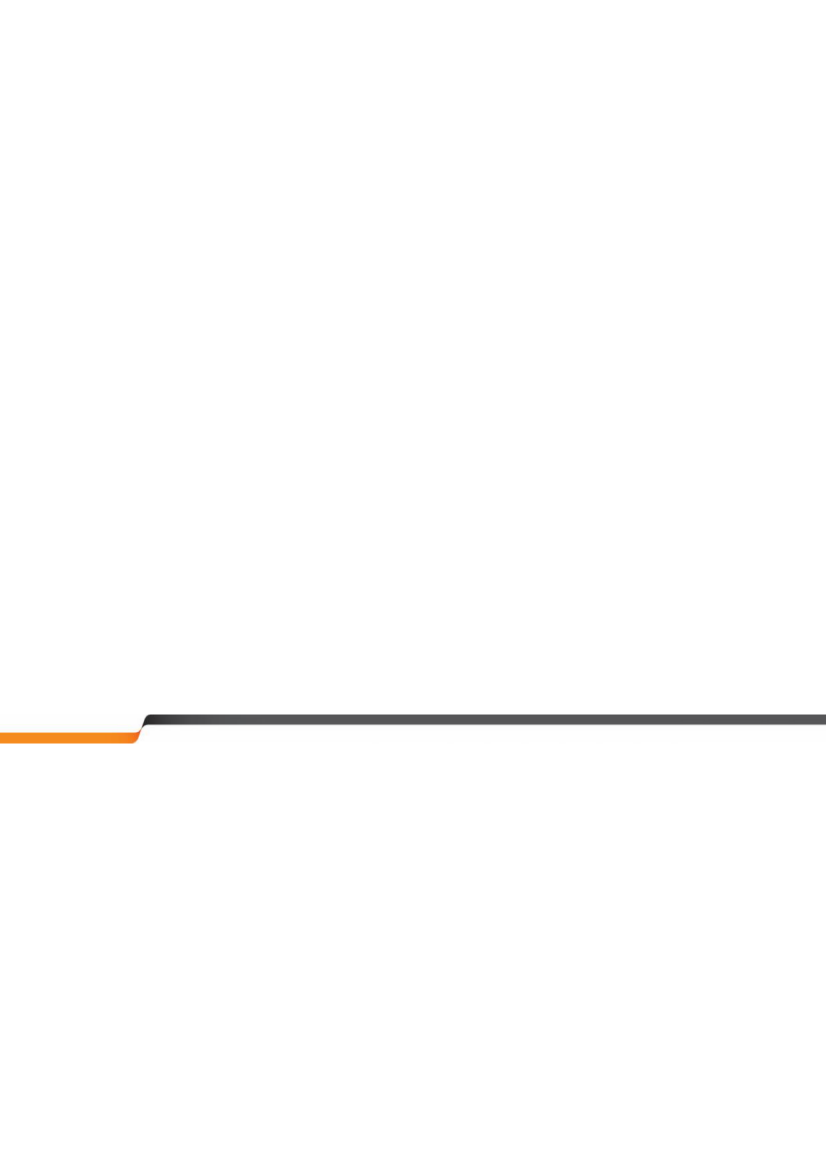
\includegraphics[width=\paperwidth,height=\paperheight,%
keepaspectratio]{viiva}%
\vfill
}}}


\makeatletter
\renewcommand{\maketitle}{
\thispagestyle{empty}
\ThisCenterWallPaper{1}{viiva}
%
\vspace*{9.5cm}
\tn{\LARGE \@author\\[0.75cm]\Huge \@title}\\[3.5cm]

\parbox{.7\linewidth}{\normalsize 
%IN FINNISH
Metropolia Ammattikorkeakoulu\\[2pt]
\tutkinto \\[2pt]
\kohjelma \\[2pt]
Insinöörityö\\[2pt]
\ddmmyyyydate\today}
%IN ENGLISH
%Helsinki Metropolia University of Applied Sciences\\[2pt]
%\metropoliadegree \\[2pt]
%\metropoliadegreeprogramme \\[2pt]
%Thesis\\[2pt]
%\ddmmyyyydate\today}%to be checked date format? 

\ThisLRCornerWallPaper{1}{metropolia}
%
\clearpage
}
\makeatother

%IN ENGLISH COMMENT THIS 3 LINES
\makepagestyle{tiivis}
\makeevenhead{tiivis}{}{}{Tiivistelmä}
\makeoddhead{tiivis}{}{}{Tiivistelmä}

\makepagestyle{abstract}
\makeevenhead{abstract}{}{}{Abstract}
\makeoddhead{abstract}{}{}{Abstract}

\begin{document}
\counterwithout{lstlisting}{chapter}

\newcommand\tn[1]{\textnormal{#1}}
\newcommand\reaction[1]{\begin{equation}\ce{#1}\end{equation}}

%page number always on the top right, clear the "chapter/section" head
\pagestyle{myheadings}
\markright{}
%clear chapter "title" foot page
\makeevenfoot{plain}{}{}{}
\makeoddfoot{plain}{}{}{}

%----------------------------------------------------------------------------------------
%	TITLE PAGE
%----------------------------------------------------------------------------------------

\maketitle
\newpage

%----------------------------------------------------------------------------------------
%    Tiivistelmä
%----------------------------------------------------------------------------------------

%IN ENGLISH COMMENT THIS SECTION
\thispagestyle{tiivis}
\ThisLRCornerWallPaper{1}{footer}
\begin{tabular}{ | p{4,7cm} | p{10,3cm} |}
  \hline
  Tekijä(t) \newline
  Otsikko \newline\newline 
  Sivumäärä \newline
  Aika
  & 
  \makeatletter
  \@author \newline 
  \otsikko \newline\newline 
  \makeatother
  \pageref{LastPage} pages + \total{chapter} appendices \newline %! if no appendices, risk to count total of chapter :D
  \pvm		
  \\ \hline
  Tutkinto & \tutkinto
  \\ \hline
  Koulutusohjelma & \kohjelma
  \\ \hline
  Suuntautumisvaihtoehto & \suuntautumis
  \\ \hline
  Ohjaaja(t) & \ohjaajat
  \\ \hline
  \multicolumn{2}{|p{15cm}|}{
  Tiivistelmä
  } \\[14cm] \hline
  Avainsanat & \avainsanat
  \\ \hline
\end{tabular}
\clearpage

%----------------------------------------------------------------------------------------
%	ABSTRACT
%----------------------------------------------------------------------------------------

\pagestyle{abstract}
\ThisLRCornerWallPaper{1}{footer}

\begin{tabular}{ | p{4,7cm} | p{10,3cm} |}
  \hline
  Author(s) \newline
  Title \newline\newline 
  Number of Pages \newline
  Date
  & 
  \makeatletter
  \@author \newline
  \@title \newline\newline
  \pageref{LastPage} pages + \total{chapter} appendices \newline %! if no appendices, risk to count total of chapter :D
  \@date
  \makeatother
  \\ \hline
  Degree & \metropoliadegree
  \\ \hline
  Degree Programme & \metropoliadegreeprogramme
  \\ \hline
  Specialisation option & \metropoliaspecialisation
  \\ \hline
  Instructor(s) & \metropoliainstructors
  \\ \hline
  \multicolumn{2}{|p{15cm}|}{
  Abstract content
  } \\[14cm] \hline
  Keywords & \metropoliakeywords
  \\ \hline
\end{tabular}
\clearpage

%----------------------------------------------------------------------------------------
%	Acknowledgement ?
%----------------------------------------------------------------------------------------
%\chapter*{Acknowledgement}
%Thanks to my cat
%\clearpage

%----------------------------------------------------------------------------------------
%	TABLE OF CONTENTS
%----------------------------------------------------------------------------------------

\makeevenhead{plain}{}{}{}
\makeoddhead{plain}{}{}{}
\pagestyle{empty} %remove page number in toc (if longer than 2 pages)
\ThisLRCornerWallPaper{1}{footer}
\tableofcontents*
\pagestyle{empty} %remove page number in toc (if longer than 1 pages)
\ThisLRCornerWallPaper{1}{footer} %add footer image (if longer than 1 page)
\clearpage
\pagestyle{plain}

%list of figure, tables comes here...


%----------------------------------------------------------------------------------------
%    Lyhenteet / Abbreviation
%----------------------------------------------------------------------------------------

\pagestyle{empty}
\ThisLRCornerWallPaper{1}{footer}
\setlength{\parskip}{1cm}
%IN FINNISH
\chapter*{Lyhenteet}
\cftaddtitleline{toc}{chapter}{Lyhenteet}{}
%IN ENGLISH
%\chapter*{Abbreviation}
%\cftaddtitleline{toc}{chapter}{Abbreviation}{}
\begin{table}[h]
\setlength{\tabcolsep}{8pt}
\renewcommand{\arraystretch}{2}
\begin{tabular}{l p{12cm}}
OMG & Oh my god\\
WTF & What the F\\
TL;DR & Too long, didn't read\\
\end{tabular}
\end{table}

\newpage

%page number always on top right; also for chapter "title" page
\pagestyle{plain}
\makeevenhead{plain}{}{}{\thepage}
\makeoddhead{plain}{}{}{\thepage}

\setcounter{page}{1} %page 1 should be Introduction

%----------------------------------------------------------------------------------------
%	CONTENT
%----------------------------------------------------------------------------------------



\chapter{Johdanto}
\chapter{Verkkotekniikat}
\section{UMTS}
UMTS (Universal Mobile Telecommunications System) on ns. kolmannen sukupolven (3G) matkapuhelinteknologia, jonka standardisointi aloitettiin 1990-luvun loppupuolella. Edellisen sukupolven GSM-tekniikkaan verrattuna UMTS tarjoaa uusien palveluiden lisäksi paremman äänenlaadun puheluissa sekä datasiirrossa huomattavasti suuremmat nopeudet. Tekniikka mahdollistaa yhtäaikaiset puhe- ja datayhteydet sekä QoS (Quality of Service) jaottelun. Tämä mahdollistaa usean eri sovelluksen käytön yhtäaikaisesti painottamalla näiden tärkeysjärjestystä eli prioriteettia. Esimerkkeinä voidaan käyttää reaaliaikaista ääni- tai videopuhelua, joka tarvitsee suuren prioriteetin ja samaan aikaan taustalla tapahtuvaa sähköpostin tarkistusta, joka tarvitsee hyvin pienen prioriteetin. 

UMTS:n 3GPP Release 99 mukainen radiotekniikka perustuu WCDMA:iin (Wideband Code Division Multiple Access). WCDMA on hajaspektritekniikka, jossa käytetään radiorajapinnan datan erotteluun koodeja sen sijaan, että käytettäisiin eri taajuuksia tai aikavälejä. Käytössä on kaksi eri koodia. 
\begin{figure}[H]
	\centering
	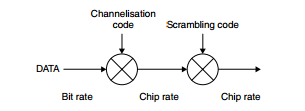
\includegraphics{umtscodes}
	\caption{Channelization ja scrambling koodien käyttö}
	\label{fig:umtscodes}
\end{figure}
Kanavointikoodia(Channelization code) käytetään downlink-suunnassa käyttäjien erotteluun tukiaseman solun alueella ja uplink-suunnassa saman laitteen kontrolli- ja datakanavien erottamiseen. Toinen käytetty koodi on sekoituskoodi (Scrambling code) jolla downlink-suunnassa erotellaan tukiasemien eri solut/sektorit ja uplink-suunnassa eri päätelaitteet. Kanavointikoodin pituus määrittää käytössä olevan bittinopeuden. Tätä kutsutaan levityskertoimeksi (Spreading factor). Kerrointa voidaan kasvattaa tai pienentää tarpeen mukaan lähetettävien kehysten välillä, joiden pituus WCDMA:ssa on 10 ms.
\begin{table}[H]
	\centering
	\caption{WCDMA datanopeudet downlink-suuntaan}
	\begin{tabularx}{.95\textwidth}{|X|X|X|X|}
		\hline
		SF & Kanavan bittinopeus (kbps)& DPDCH kanavan bittinopeusalue (kbps) & Käyttäjän maksimi bittinopeus (arvio) \\
    		\hline
		512 & 15 & 3-6 & 1-3 kbps \\
		256 & 30 & 12-24 & 6-12 kbps \\
		128 & 60 & 42-51 & 20-24 kbps \\
		64 & 120 & 90 & 45 kbps \\
		32 & 240 & 210 & 105 kbps \\
		16 & 480 & 432 & 215 kbps \\
		8 & 960 & 912 & 456 kbps \\
		4 & 1920 & 1872 & 936 kbps \\
		4, 3 rinnakkaisella koodilla & 5760 & 5616 & 2.8 Mbps \\
    		\hline
	\end{tabularx}
	\label{table:wcdmadatanopeudet}
\end{table}
Käytännön WCDMA datanopeutta rajoittavat 3GPP Release 99:ssä määritellyt päätelaiteluokat joita on yhteensä kuusi. 
\begin{table}[H]
	\centering
	\caption{WCDMA päätelaiteluokat}
	\begin{tabularx}{.95\textwidth}{|X|X|}
		\hline
		Luokka & Käyttötarkoitus \\
    		\hline
		32 kbps luokka & Perus puhekäyttö, rajoitettu data 32 kbps asti. \\
    		\hline
		64 kbps luokka & Puhe ja datakäyttö. Yhtäaikainen AMR puhe ja data. \\
    		\hline
		144 kbps luokka & Lisää esim. mahdollisuuden videopuheluihin. \\
    		\hline
		384 kbps luokka & Pykälää nopeampi. Multicode-tuki, pystyy hyödyntämään useita koodeja yhtäaikaisesti.  \\
    		\hline
		768 kbps luokka & Edelleen pykälää nopeampi. Suunniteltu välimalliksi. \\
    		\hline
		2 Mbps luokka & Huippumalli. Nopeus määritelty downlink-suuntaan. \\
		\hline
	\end{tabularx}
	\label{table:wcdmapaatelaiteluokat}
\end{table}
Jo UMTS:n standardisointivaiheessa haluttiin taata hyvä päivitettävyys vanhoista GSM verkoista. Tästä seurasi se, että UMTS käyttää samaa runkoverkkorakennetta. Kuvassa \ref{fig:umtscore} tämä merkitty CN (Core Network).
\begin{figure}[H]
	\centering
	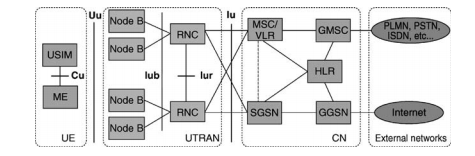
\includegraphics{umtscore}
	\caption{UMTS verkon rakenne}
	\label{fig:umtscore}
\end{figure}
Tässä MSC/VLR (Mobile Services Switching Center/Visitor Location Register) hoitaa piirikytkentäisten puhelujen yhdistämisen ja pitää kirjaa MSC:n alueella olevista päätelaitteista (UE). HLR (Home Location Register) pitää sisällään käyttäjien palveluprofiilin, joka sisältää kaiken laskutuksesta puhelunohjaukseen yms, sekä sijaintitiedon MSC/VLR ja/tai SGSN tasolla. GMSC (Gateway MSC) toimii yhdyskäytävänä muihin piirikytkentäisiin verkkoihin. 

Pakettiliikennettä hoitavat SGSN (Serving GPRS (General Packet Radio Service) Support Node), joka vastaa puheluihin käytettyä MSC/VLR-yksikköä hoitaen pakettidatan kytkennän ja GGSN (Gateway GPRS Support Node), joka toimii vastaavasti yhdyskäytävänä pakettidataa käyttäviin ulkoisiin järjestelmiin, esim. IP verkkoihin ja sitä kautta Internetiin. 

Radioverkkoa kuvassa \ref{fig:umtscore} edustaa UTRAN (UMTS Terrestrial Radio Access Network), joka koostuu RNC-yksiköistä (Radio Network Controller) sekä tukiasemista (Node B). RNC:t kontrolloivat radioverkon resursseja omalla alueellaan, johon voi kuulua useita tukiasemia. Se on myös vastuussa pääsynhallinnasta (Admission Control), koodien määrittelystä sekä yleisestä liikenteen kontrolloinnista. Tukiaseman tehtävä on kontrolloida fyysistä radiorajapintaa ja radioresursseja UE:n tehonsäädön muodossa. 

GSM-radioverkkoon verrattuna uutta UTRAN:n rakenteessa on Iur-rajapinta, joka mm. mahdollistaa eri valmistajien RNC:iden välisen kommunikaation. Rajapintaa käytetään myös liikenteen reitittämiseen tilanteissa joissa päätelaite siirtyy RNC:n alueelta toiselle.

 {\color{red}Tähän joku 3GPP Roadmap umts:n kehityksestä.}

Datanopeuksien kehittämiseksi on UMTS:iin on määritelty ajan myötä uusia tekniikoita, joilla parannetaan siirtonopeuksia radioverkossa. Ensimmäinen parannus julkaistiin 3GPP Release 5:n myötä, jossa määriteltiin HSDPA (High Speed Downlink Packet Access). Tätä varten radiorajapintaan määriteltiin uudet fyysisen kerroksen signallinti- ja liikennekanavat, parempi virheenkorjaustekniikka parantamaan verkon vasteaikaa ja tehokkaampi modulaatio, jolla pystytään siirtämään enemmän bittejä symbolia kohti. 

Kanavan resurssit on jaettu kanavointikoodein joista 16:ta voidaan varsinaisen dataliikenteen käyttöön antaa 15. Hyödyntämällä kaikki koodit ja käyttämällä QPSK:n sijaan 16-QAM modulaatiota pystytään downlink-suunnan teoreettista huippunopeutta kasvattamaan 14 Mbit/s asti. 

\section{LTE}

\chapter{Mittalaitteet ja sovellukset}
Mittauksia varten hankittiin liittymä, päätelaite sekä antenni. Valinnassa suurimmaksi kriteeriksi asetettiin monikäyttöisyys, sillä laitteita oli tarkoitus käyttää myös mittausten jälkeen aktiivisesti normaalikäytössä.
\section{Liittymä}
Liittymäksi valittiin Saunalahden Mobiililaajakaista 4G 50 Mbit/s varianttina. Liittymän valintaan vaikutti jo olemassa oleva kyseisen operaattorin puheliittymä, sekä hinta. Täyden nopeuden liittymälle (100 Mbit/s) ei nähty tarvetta normaalikäytön, eikä suoritettavien mittauksienkaan kannalta.

Hinnan sekä nopeuden lisäksi peruskäyttäjän kannattaa tutkia operaattoreiden kuuluvuuskarttoja mikäli liittymää on tarkoitus käyttää pääasiassa esimerkiksi kotona. Näin voidaan etukäteen kartoittaa sijaitseeko pääasiallinen käyttökohde kyseisen operaattorin kuuluvuusalueella ja välttää täysin kuuluvuusalueen ulkopuolelle jääminen.
\section{Päätelaite}
\begin{figure}[H]
	\centering
	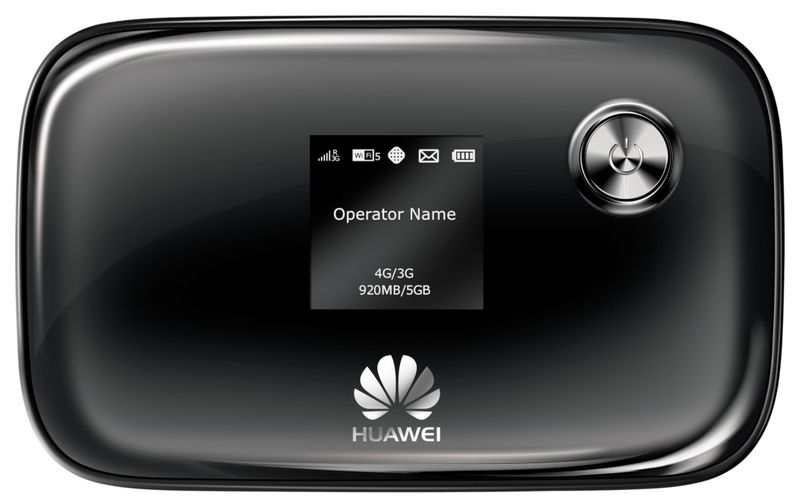
\includegraphics{e5776etu}
	\caption{Huawei E5776 mobiilireititin}
	\label{fig:e5776etu}
\end{figure}

Päätelaitteeksi valittiin operaattorin sen hetken valikoimasta Huawei E5776 mobiilireititin. Kyseinen päätelaite kykenee parhaimmillaan LTE verkossa 150 Mbit/s lataus- ja 50 Mbit/s lähetysnopeuteen sekä UMTS verkossa DC-HSPA+ tekniikalla 42 Mbit/s lataus ja 20 Mbit/s lähetysnopeuteen. Reititintä voidaan käyttää joko WiFi yhdyspisteenä tai suoraan USB kaapelilla tietokoneeseen kytkettynä. Langatonta lähiverkkoa käytettäessä latausnopeus on rajattu 65 Mbit/s.

Vaikka reitittimestä löytyvät sisäiset 2x2 MIMO antennit, on siinä vain yksi ulkoinen antenniliitäntä. Suurinta mahdollista tiedonsiirtonopeutta tavoiteltaessa kannattaa valita päätelaite, jossa on mahdollista hyödyntää MIMO-tekniikkaa myös ulkoisilla antenneilla.

Reitittimessä on myös sisäinen akku, joka lisää entisestään laitteen monikäyttöisyyttä.
\section{Antenni}

Ulkoiseksi antenniksi valittiin mobiiliverkon antenneihin erikoistuneen yrityksen valikoimasta CSG Networksin laajakaistainen ympärisäteilevä piiska magneettikiinnityksellä. Antenni toimii parhaiten taajuuksilla 824-960MHz, 1710-1990MHz ja 2170MHz. Suomessa käytössä olevat 800MHz LTE taajuudet ovat vielä suhteellisen lähellä antennin parhainta toiminta-aluetta, mutta 2600MHz kaista jää ikävästi pois tästä. Tämän ei kuitenkaan katsottu haittaavan suunniteltua käyttöä.

Magneettikiinnitys yhdessä akkukäyttöisen reitittimen kanssa mahdollistaa monipuoliset käyttömahdollisuudet niin kiinteissä kuin liikkuvissakin käyttökohteissa.
\begin{figure}[H]
	\centering
	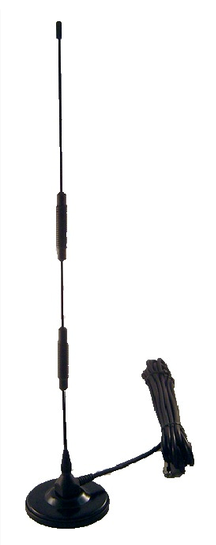
\includegraphics[scale=0.5]{antennapic}
	\caption{Magneettijalkainen piiska-antenni}
	\label{fig:antennapic}
\end{figure}

Antennin lisäksi hankittiin samasta liikkeestä adapteri reitittimen TS9 ja antennin SMA-liitännän välille. Adapteria yleensä tarvitaan, koska päätelaitteiden pieni koko asettaa rajoitteita antenniliittimille.

\section{Mittaussovellus}
%Digitaalisessa tiedonsiirrossa suurin mahdollinen tiedonsiirtonopeus voidaan katsoa määriteltävän Shannon-Hartley kaavan mukaisesti, jossa kanavan bittinopeutta rajoittavat käytetty kaistanleveys sekä signaalikohinasuhde. Käytännön sovelluksissa täytyy ottaa huomioon vielä että signallointi eli merkinanto, virheenkorjaus sekä datan koodaus ovat pois hyötykuorman määrästä.

Käytännössä mobiiliverkoissa tekniikan asettamaa suurinta nopeutta rajoittavat käytetyn kanavan voimakkuus sekä siellä esiintyvien häiriöiden määrä. Voimakkaassa kanavassa voi esiintyä siinä määrin häiriöitä, että tiedonsiirtonopeus kärsii huomattavasti, mutta myös vastaavasti heikossa kanavassa, jossa ei ole juurikaan häiriöitä, voidaan saavuttaa kohtuullisen hyviäkin nopeuksia. Yleensä kuitenkin heikko kanava on alttiimpi häiriöille sekä virheilyille, jolloin saavutettu nopeus jää vaatimattomammaksi.

Oikeilla mittalaitteilla voidaan päätelaitteesta mitata hyvinkin tarkasti päätelaitteen, radioverkon sekä myös tuotteesta riippuen palveluiden toimivuutta. Valitettavasti kyseiset laitteet on hinnoiteltu tavallisen käyttäjän ulottumattomiin, joten niitä ei tässä tapauksessa voitu käyttää.

Tavallisesta päätelaitteesta on pienellä varauksella mahdollista saada ulos joitakin tässä tapauksessa kiinnostavia mittausarvoja. Tämä varaus johtuu lähinnä julkisesti saatavissa olevan dokumentoinnin puutteesta. Vaikka internetistä nykypäivänä löytyy tietoa lähes kaikesta, on joistain aiheista lähes mahdoton löytää ajantasaista tietoa. Tässäkin tapauksessa jouduttiin turvautumaan hieman vanhempaan ja vieläpä eri päätelaitteen dokumentaatioon. 

Mikäli päätelaitteessa on web-hallinta, saattaa siellä olla jotain tietoja näkyvillä. Tämä kelpaa mainiosti satunnaiseen seurantaan, mutta kun haluttiin kerätä dataa tarkemmin ja automatisoidusti, jäi vaihtoehdoksi käyttää joko Huawei:n web API:a tai sarjalinkin ylitse lähetettäviä AT-komentoja. Ensin mainitusta on vieläkin vähemmän dokumentteja löydettävissä kuin jälkimmäisestä, joten päädyttiin jälkimmäiseen. Komennot perustuvat Hayesin komentosarjaan joka kehitettiin 1980-luvulla. Lähes kaikkia nykyaikaisia modeemeja on mahdollista ohjata tähän perustuvilla komennoilla. 
Dokumentteja selailemalla ja kokeilemalla komentoja saatiin selville, mitkä komennoista antaisivat mahdollisesti hyödyllistä tietoa.

\begin{table}[H]
	\centering
	\caption{CURC-komento}
	\begin{tabularx}{.95\textwidth}{|p{3.5cm}|X|}
		\hline
		Komento & Tuloste \\
    		\hline
		AT\^{}CURC=<mode> & OK \\
		\hline
	\end{tabularx}
	\label{table:atkomento_curc}
\end{table}
CURC-komennolla asetetaan automaattinen raportointi päälle tai pois. Tällöin modeemi tulostaa automaattisesti meitä kiinnostavan \^{}DSFLOWRPT-komennon listauksen tietyin väliajoin.
\begin{table}[H]
	\centering
	\caption{SYSINFOEX-komento}
	\begin{tabularx}{.95\textwidth}{|p{3.5cm}|X|}
		\hline
		Komento & Tuloste \\
    		\hline
		AT\^{}SYSINFOEX & \textless srv\_status\textgreater , \textless srv\_domain\textgreater , \textless roam\_status\textgreater , \textless sim\_state\textgreater , \textless lock\_state\textgreater , \textless sysmode\textgreater , \textless sysmode\_name\textgreater \textless submode\textgreater , \textless submode\_name\textgreater \\
		\hline
	\end{tabularx}
	\label{table:atkomento_sysinfoex}
\end{table}
SYSINFOEX-komennolla saadan paljon hyödyllistä tietoa modeemin toiminnasta. 
\begin{table}[H]
	\centering
	\caption{ANQUERY-komento}
	\begin{tabularx}{.95\textwidth}{|p{3cm}|X|}
		\hline
		Komento & Tuloste \\
    		\hline
		AT\^{}ANQUERY? & \textless rscp\textgreater , \textless ecio\textgreater , \textless rssi\textgreater , \textless antenna\_level\textgreater , \textless rsrp\textgreater , \textless rsrq\textgreater \\
		\hline
	\end{tabularx}
	\label{table:atkomento_anquery}
\end{table}
Selitä komennosta hyödynnettävä tieto
\begin{table}[H]
	\centering
	\caption{CREG-komento}
	\begin{tabularx}{.95\textwidth}{|p{3cm}|X|}
		\hline
		Komento & Tuloste \\
    		\hline
		AT+CREG? & \textless n\textgreater , \textless stat\textgreater [ , \textless lac\textgreater , \textless ci\textgreater ] \\
		\hline
	\end{tabularx}
	\label{table:atkomento_creg}
\end{table}
Selitä komennosta hyödynnettävä tieto
\begin{table}[H]
	\centering
	\caption{DSFLOWRPT-komento}
	\begin{tabularx}{.95\textwidth}{|p{3cm}|X|}
		\hline
		Komento & Tuloste \\
    		\hline
		AT\^{}DSFLOWRPT & \textless curr\_ds\_time\textgreater , \textless tx\_rate\textgreater , \textless rx\_rate\textgreater , \textless curr\_tx\_flow\textgreater , \textless curr\_rx\_flow\textgreater , \textless qos\_tx\_rate\textgreater , \textless qos\_rx\_rate\textgreater \\
		\hline
	\end{tabularx}
	\label{table:atkomento_dsflowrpt}
\end{table}
Selitä komennosta hyödynnettävä tieto

AT+CLAC komennolla voidaan listata kaikki laitteen tukemat komennot, joiden joukosta löytyi nimien perusteella muitakin mielenkiintoisia komentoja, joita olisi ollut mielenkiintoista seurata. Dokumentaatioista ei kuitenkaan varmuudella löytynyt tietoa arvoista, jotka komennot tulostavat, joten näitä ei käytetty mittauksien tulkinnassa.

\begin{figure}[H]
	\centering
	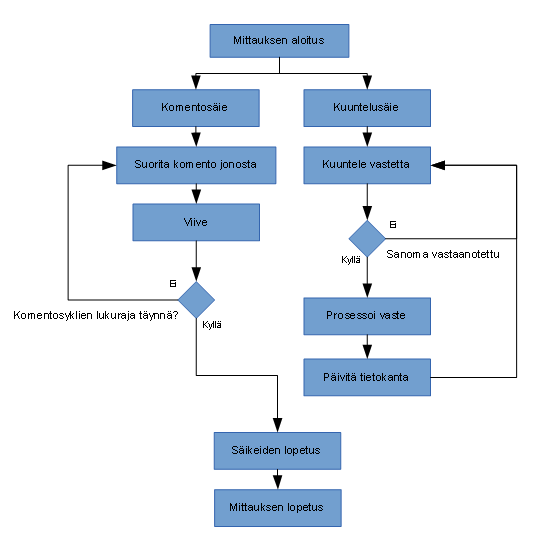
\includegraphics{mittausohjelma_flowchart}
	\caption{Mittausohjelman vuokaavio}
	\label{fig:mittausohjelma_flowchart}
\end{figure}


Mittaussovellus toteutettiin Python-kielellä. Sovellus käynnistää kaksi säiettä, joista toinen hoitaa komentojen lähettämisen modeemille ja toinen vastaussanomien käsittelyn ja datan tallentamisen SQLite:llä toteutettuun tietokantaan. Sarjaliikenteen käsittelyyn käytetään PySerial moduulia. Graafinen käyttöliittymä toteutettiin PyQt kirjastoa käyttäen.

\begin{figure}[H]
	\centering
	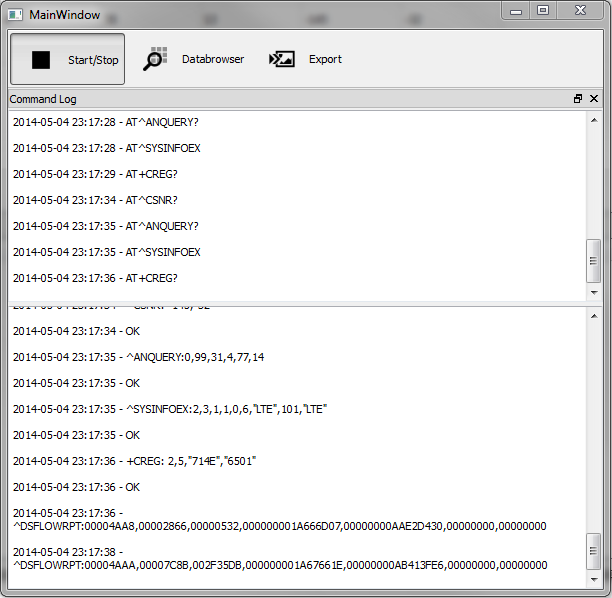
\includegraphics[scale=0.75]{loggeri}
	\caption{Mittausohjelman käyttöliittymä}
	\label{fig:loggeri}
\end{figure}
Sovelluksen tueksi kirjoitettiin PHP-kielellä mittausdatan visualisoiva web-sivu, jossa käyrien piirtäminen toteutettiin Google Graph API:lla.


\chapter{Mittaukset}
\section{Mittausprosessi}
\begin{figure}[H]
	\centering
	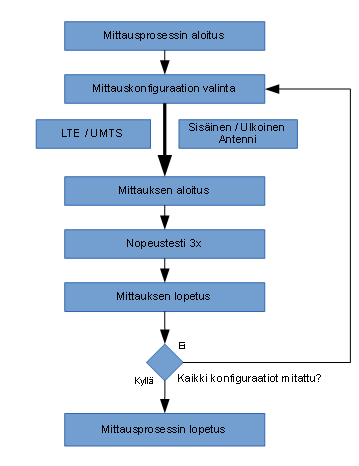
\includegraphics[scale=1.0]{mittausprosessi_flowchart}
	\caption{Mittausprosessin vuokaavio}
	\label{fig:mittausprosessi_flowchart}
\end{figure}
Mittausprosessi aloitettiin valitsemalla kohteessa sijainti, jossa päätelaite normaalisti käytettäessä voisi sijaita. Tämän jälkeen suoritettiin neljä mittaussarjaa, joista ensimmäiset kaksi ilman ulkoista antennia, ja jälkimmäiset ulkoisen antennin kanssa. Päätelaite lukittiin vuorotellen UMTS ja LTE verkkoon. 

Kun yhteys verkkoon muodostui, käynnistettiin mittaus sovelluksessa. Tämän jälkeen verkkoa kuormitettiin speedtest.net:n nopeustestin automaattiasetuksilla kolme kertaa peräkkäin. Kun nopeustestit on ajettu loppuu, lopetetaan mittaus ja tallennetaan tiedot tietokantaan. Ym. prosessi toistettiin kaikille neljälle testikonfiguraatiolle.

\section{Mittauskohde 1}
\section{Mittauskohde 2}

\chapter{Johtopäätökset}

%----------------------------------------------------------------------------------------
%   BIBLIOGRAPHY 
%----------------------------------------------------------------------------------------

\bibliographystyle{vancouver}
%line space
%\singlespacing %removed otherwise the appendix are also single space
\begin{flushleft}
\begin{singlespacing}
\bibliography{biblio}
\end{singlespacing}
\end{flushleft}

%for conting the pages
\label{LastPage}~


%----------------------------------------------------------------------------------------
%   APPENDICES 
%----------------------------------------------------------------------------------------
%avoid that the last page of bib get appendix header
\clearpage
%start appendix
\appendix
%no page number for appendix in table of content
\addtocontents{toc}{\cftpagenumbersoff{chapter}}
%appendix sections and subsections not in table of content
\settocdepth{chapter}
%add "Appendices" in the table of content
\addappheadtotoc
%force smaller vertical spacing in table of content
%!!! There can be some fun depending if the appendices have (sub)sections or not :D
% You will have to play with these numbers and eventually copy the \pretocmd line on before some \chapter and force another number.
\addtocontents{toc}{\vspace{11pt}}
\pretocmd{\chapter}{\addtocontents{toc}{\protect\vspace{-24pt}}}{}{}

%have Appendix 1 (instead of Appendix A)
\renewcommand{\thechapter}{\arabic{chapter}} 

%each appendix restart page num to one
\setcounter{page}{1}
%special counter for appendix TODO: this is a ugly quick hack :( Should find a better way to count the page per appendix.
\newtotcounter{appx1}
%overwrite the header
\makeevenhead{plain}{}{}{Appendix \thechapter \\ \thepage (\stepcounter{appx1}\total{appx1})}
\makeoddhead{plain}{}{}{Appendix \thechapter \\ \thepage (\stepcounter{appx1}\total{appx1})}
%LIITTEET


\end{document}
